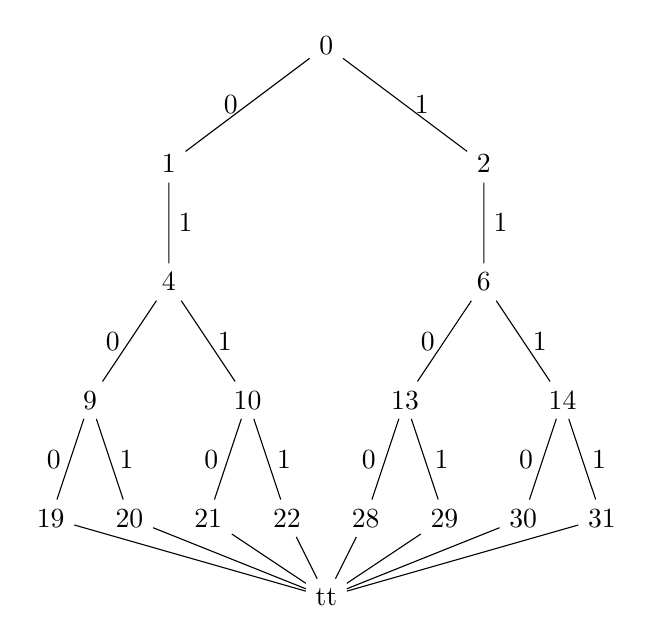
\begin{tikzpicture}
  [
    level 1/.style = {sibling distance = 4cm},
    level 2/.style = {sibling distance = 4cm},
    level 3/.style = {sibling distance = 2cm},
    level 4/.style = {sibling distance = 1cm},
  ]

  \node (root) at (0,0) {0}
  child {node {1}
      child {
          node {4}
          child {node {9}
              child {node {19}
                  edge from parent node [left] {0}}
              child {node {20}
                  edge from parent node [right] {1}}
              edge from parent node [left] {0}}
          child {node {10}
              child {node {21}
                  edge from parent node [left] {0}}
              child {node {22}
                  edge from parent node [right] {1}}
              edge from parent node [right] {1}}
          edge from parent node [right] {1}}
      edge from parent node [left] {0}
    }
  child {node {2}
      child {node {6}
          child {node {13}
              child {node {28}
                  edge from parent node [left] {0}}
              child {node {29}
                  edge from parent node [right] {1}}
              edge from parent node [left] {0}}
          child {node {14}
              child {node {30}
                  edge from parent node [left] {0}}
              child {node {31}
                  edge from parent node [right] {1}}
              edge from parent node [right] {1}}
          edge from parent node [right] {1}}
      edge from parent node [right] {1}
    };

  \node (bottomnode) at (0,-7) {tt};

  \foreach \w in {1,2}{
      \foreach \x in {1,2} {
          \foreach \y in {1, 2}{
              \draw (root-\w-1-\x-\y) -- (bottomnode);
            }
        }
    }

\end{tikzpicture}